% --------------------------------------------------------
% DEFINIÇÕES DO DOCUMENTO
% --------------------------------------------------------

\documentclass[
	% -- opções da classe memoir --
	12pt,				% tamanho da fonte
	openright,			% capítulos começam em pág ímpar (insere página vazia caso preciso)
	oneside,			% para impressão em verso e anverso. Oposto a twoside
	a4paper,			% tamanho do papel.
	% -- opções da classe abntex2 --
	%chapter=TITLE,		% títulos de capítulos convertidos em letras maiúsculas
	%section=TITLE,		% títulos de seções convertidos em letras maiúsculas
	%subsection=TITLE,	% títulos de subseções convertidos em letras maiúsculas
	%subsubsection=TITLE,% títulos de subsubseções convertidos em letras maiúsculas
	% -- opções do pacote babel --
	english,			% idioma adicional para hifenização
	french,				% idioma adicional para hifenização
	spanish,			% idioma adicional para hifenização
	brazil,				% o último idioma é o principal do documento
	]{lib/abntex2}


% --------------------------------------------------------
% PACOTES
% --------------------------------------------------------
\usepackage{pdfpages}
\usepackage{cmap}				% Mapear caracteres especiais no PDF
\usepackage{helvet}
%\usepackage{lmodern}			% Usa a fonte Latin Modern
\usepackage[T1]{fontenc}		% Selecao de codigos de fonte.
\usepackage[utf8]{inputenc}		% Codificacao do documento (conversão automática dos acentos)
\usepackage{lastpage}			% Usado pela Ficha catalográfica
\usepackage{indentfirst}		% Indenta o primeiro parágrafo de cada seção.
\usepackage{color}				% Controle das cores
\usepackage{graphicx}			% Inclusão de gráficos
\usepackage{lipsum}				% para geração de dummy text
\usepackage{courier}            % fonte courier

\let\printglossary\relax
\let\theglossary\relax
\let\endtheglossary\relax
\usepackage{lib/update-abntex}

\usepackage[brazilian,hyperpageref]{}	 % Paginas com as citações na bibl
\usepackage{microtype} 

\usepackage{silence}
%Disable all warnings issued by latex starting with "You have..."
\WarningFilter{latex}{You have requested package}
\usepackage[alf, abnt-etal-list=0 ]{lib/abntex2cite}	% Citações padrão ABNT
\usepackage[br]{lib/nicealgo}       % Pacote para criação de algoritmos
\usepackage{lib/customizacoes}      % Pacote de customizações do abntex2

\usepackage{listings}
\usepackage[normalem]{ulem} % Strikethrough package

% --------------------------------------------------------
% CONFIGURAÇÕES DE PACOTES
% --------------------------------------------------------

% Configurações do pacote listing
\renewcommand{\lstlistingname}{Código} %Mudança no caption do listing para Código
\renewcommand{\lstlistlistingname}{Lista de códigos} %Mudança no caption da lista de listings.

% Contagem de códigos sem incluir o número do capítulo
\usepackage{chngcntr}
\AtBeginDocument{\counterwithout{lstlisting}{chapter}}


% Configurações do pacote backref
\renewcommand{\familydefault}{\sfdefault}
% Usado sem a opção hyperpageref de backref
% \renewcommand{\backrefpagesname}{Citado na(s) página(s):~}
% Texto padrão antes do número das páginas
% \renewcommand{\backref}{}
% Define os textos da citação
% \renewcommand*{\backrefalt}[4]{
% 	\ifcase #1 %
% 		Nenhuma citação no texto.%
% 	\or
% 		Citado na página #2.%
% 	\else
% 		Citado #1 vezes nas páginas #2.%
% 	\fi}%


% --------------------------------------------------------
% INFORMAÇÕES DE DADOS PARA CAPA E FOLHA DE ROSTO
% --------------------------------------------------------

\titulo{Explorando Algoritmos de Compressão de Dados: Teoria, Implementação e Desempenho}
\autor{Gustavo Yujii Silva Kadooka}
\local{Bauru}
\data{Novembro/2025}
\orientador{Profa. Dra. Andréa Carla Gonçalves Vianna}
\instituicao{%
  Universidade Estadual Paulista ``Júlio de Mesquita Filho''
  \par
  Faculdade de Ciências
  \par
  Ciência da Computação}
\tipotrabalho{Trabalho de Conclusão de Curso}
\preambulo{Trabalho de Conclusão de Curso em Ciência da Computação apresentado ao Departamento de Computação da Universidade Estadual Paulista ``Júlio de Mesquita Filho'', Faculdade de Ciências, Campus Bauru.}


% --------------------------------------------------------
% CONFIGURAÇÕES PARA O PDF FINAL
% --------------------------------------------------------

% alterando o aspecto da cor azul
\definecolor{blue}{RGB}{41,5,195}


% informações do PDF
\makeatletter
\hypersetup{
     	%pagebackref=true,
		pdftitle={\@title},
		pdfauthor={\@author},
    	pdfsubject={\imprimirpreambulo},
	    pdfcreator={LaTeX with abnTeX2},
		pdfkeywords={abnt}{latex}{abntex}{abntex2}{trabalho acadêmico},
		colorlinks=true,       		% false: boxed links; true: colored links
    	linkcolor=black,          	% color of internal links
    	citecolor=black,        		% color of links to bibliography
    	filecolor=magenta,      		% color of file links
		urlcolor=black,
		bookmarksdepth=4
}
\makeatother


% ---
% Posiciona figuras e tabelas no topo da página quando adicionadas sozinhas
% em um página em branco. Ver https://github.com/abntex/abntex2/issues/170
\makeatletter
\setlength{\@fptop}{5pt} % Set distance from top of page to first float
\makeatother
% ---

% ---
% Possibilita criação de Quadros e Lista de quadros.
% Ver https://github.com/abntex/abntex2/issues/176
%
\newcommand{\quadroname}{Quadro}
\newcommand{\listofquadrosname}{Lista de quadros}

\newfloat[chapter]{quadro}{loq}{\quadroname}
\newlistof{listofquadros}{loq}{\listofquadrosname}
\newlistentry{quadro}{loq}{0}

% configurações para atender às regras da ABNT
\setfloatadjustment{quadro}{\centering}
\counterwithout{quadro}{chapter}
\renewcommand{\cftquadroname}{\quadroname\space} 
\renewcommand*{\cftquadroaftersnum}{\hfill--\hfill}

\setfloatlocations{quadro}{hbtp}
% ---


% --------------------------------------------------------
% ESPAÇAMENTOS ENTRE LINHAS E PARÁGRAFOS
% --------------------------------------------------------

% O tamanho do parágrafo é dado por:
\setlength{\parindent}{1.3cm}

% Controle do espaçamento entre um parágrafo e outro:
\setlength{\parskip}{0.2cm}


% --------------------------------------------------------
% COMPILANDO O ÍNDICE
% ---------------------------------------------------
\makeindex
% ---
 
% ---
% GLOSSARIO
% ---
\makeglossaries
% ---
% Exemplo de configurações do glossairo
\renewcommand*{\glsseeformat}[3][\seename]{\textit{#1}  
 \glsseelist{#2}}
% ---
 
% --------------------------------------------------------
% INÍCIO DO DOCUMENTO
% --------------------------------------------------------

\begin{document}

% Seleciona o idioma do documento (conforme pacotes do babel)
\selectlanguage{brazil}

% Retira espaço extra obsoleto entre as frases.
\frenchspacing


% --------------------------------------------------------
% ELEMENTOS PRÉ-TEXTUAIS
% --------------------------------------------------------

% Capa
\imprimircapa

% Folha de rosto
% (o * indica que haverá a ficha bibliográfica)
\imprimirfolhaderosto*

% Inserir a ficha bibliografica
\begin{fichacatalografica}
    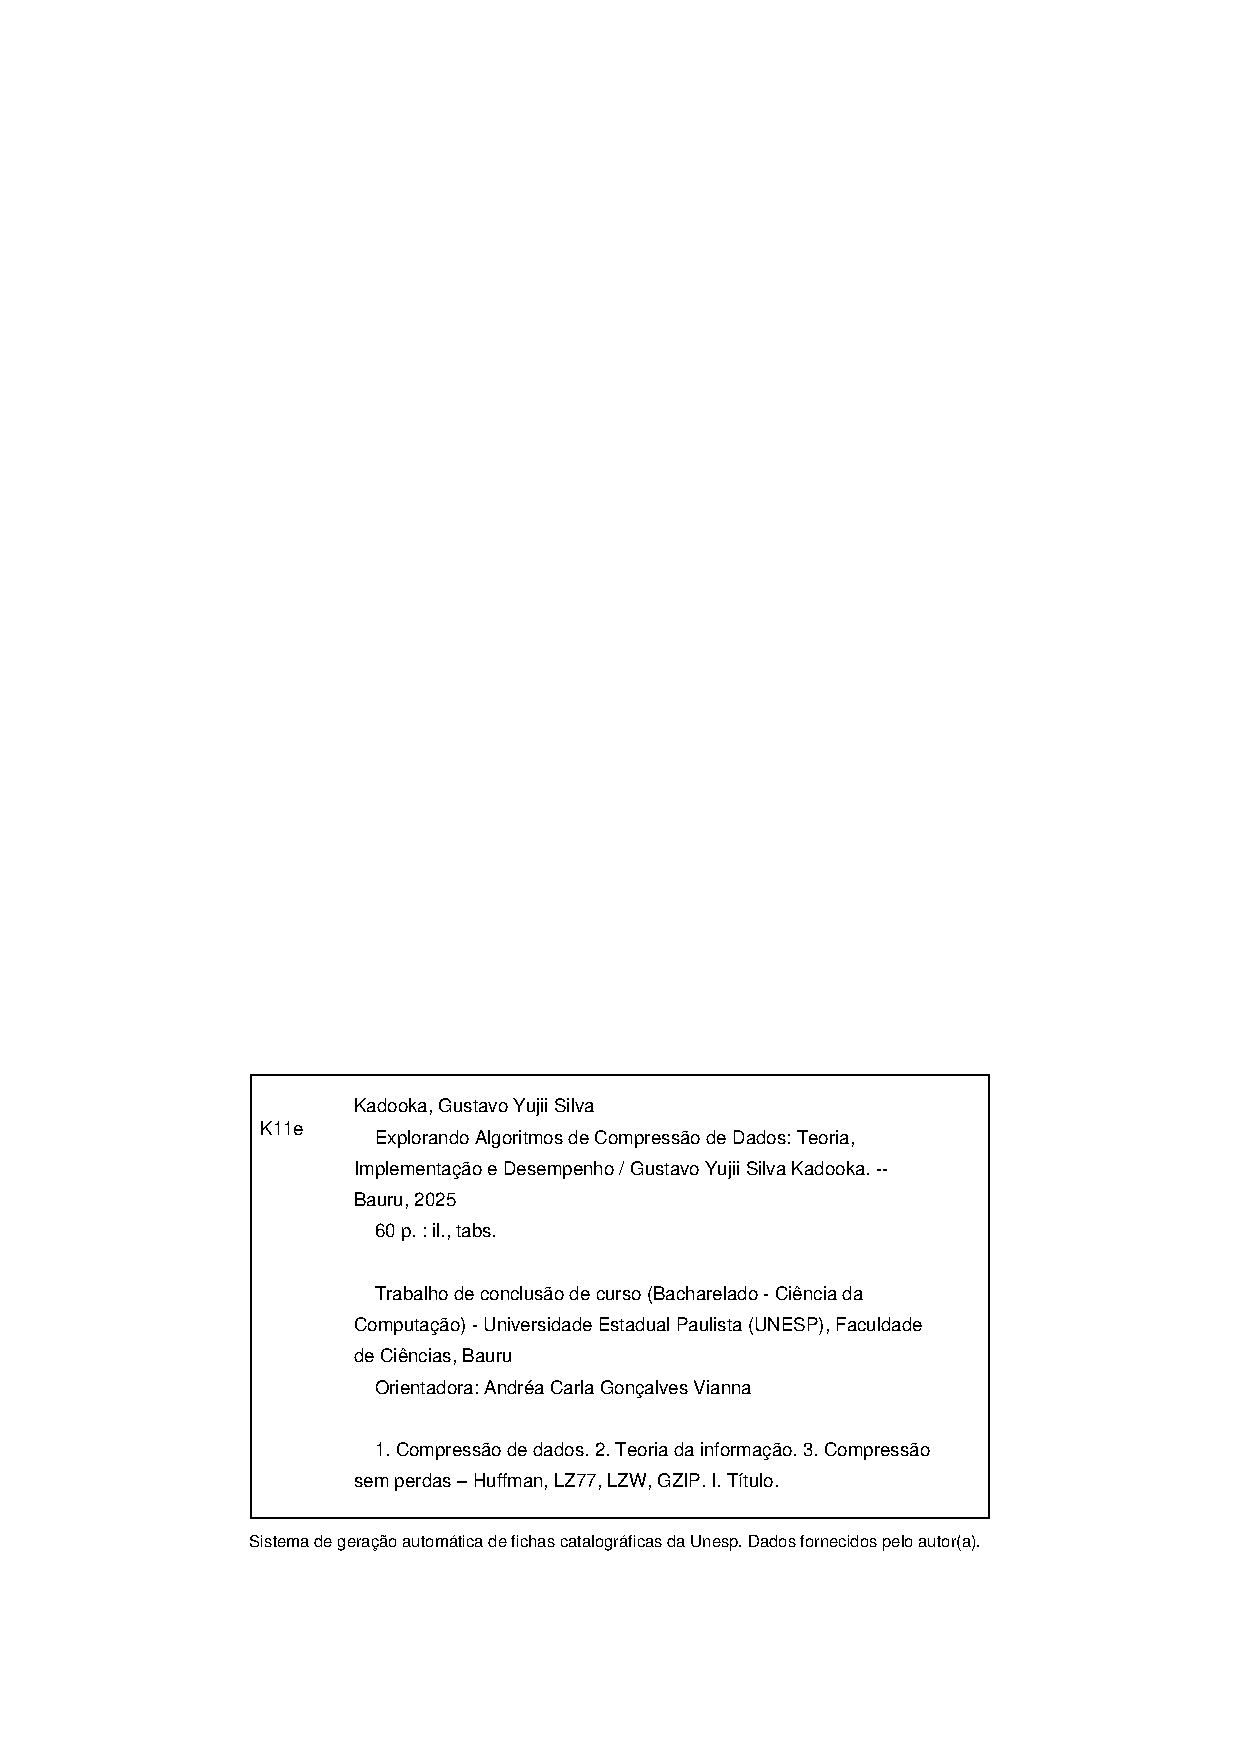
\includepdf[pages=1,offset=0cm 0cm,scale=1]{figs/ficha_catalografica.pdf}
\end{fichacatalografica}

% Inserir folha de aprovação
\begin{folhadeaprovacao}
	\begin{center}
		{\ABNTEXchapterfont\large\imprimirautor}
		\vspace*{\fill}\vspace*{\fill}
		\begin{center}
			\ABNTEXchapterfont\bfseries\Large\imprimirtitulo
		\end{center}
		\vspace*{\fill}
		\hspace{.45\textwidth}
		\begin{minipage}{.5\textwidth}
			\imprimirpreambulo
		\end{minipage}%
		\vspace*{\fill}
	\end{center}
	\center Banca Examinadora
	\assinatura{\textbf{\imprimirorientador} \\ Orientador\\
		Universidade Estadual Paulista ``Júlio de Mesquita Filho''\\
		Faculdade de Ciências \\
	Departamento de Ciência da Computação}
	\assinatura{\textbf{Professor Convidado 1} \\
		Universidade Estadual Paulista ``Júlio de Mesquita Filho''\\
		Faculdade de Ciências \\
	Departamento de Ciência da Computação}
	\assinatura{\textbf{Professor Convidado 2} \\
		Universidade Estadual Paulista ``Júlio de Mesquita Filho''\\
		Faculdade de Ciências \\
	Departamento de Ciência da Computação}
	\begin{center}
		\vspace*{0.5cm}
		\par
		{Bauru, 11 de novembro de 2025.}
		\vspace*{1cm}
	\end{center}
\end{folhadeaprovacao}

% Dedicatória
\begin{dedicatoria}
	\vspace*{\fill}
	\begin{flushright}
        \textit{À minha amada família, fonte inesgotável de inspiração e força.} 
	\end{flushright}
\end{dedicatoria}

% Agradecimentos
\begin{agradecimentos}
    Agradeço à Universidade Estadual Paulista ``Júlio de Mesquita Filho'' -- Faculdade de Ciências, Campus de Bauru --,
    por ter sido o espaço onde pude me desenvolver como estudante, profissional e indivíduo. Sou grato a todos os
    professores e funcionários da instituição pelo conhecimento compartilhado e pelo apoio ao longo da graduação.
    
    À minha orientadora, Profa. Dra. Andréa Carla Gonçalves Vianna, pela disponibilidade, paciência diante das dificuldades 
    e por acreditar no meu potencial durante o desenvolvimento deste trabalho.

    Aos meus colegas de curso, que estiveram presentes ao longo desta jornada, dividindo aprendizados,
    desafios e conquistas. O convívio e a troca de experiências tornaram a caminhada mais leve e significativa.

    À minha irmã Gabriely, pelas palavras de incentivo e carinho em todos os momentos, mesmo nos mais difíceis.

    E, com o meu mais profundo e sincero agradecimento, menciono especialmente meus pais -- Flávia e Silvio
    --, por todo o apoio emocional, pelos ensinamentos de vida, pela confiança depositada em mim e por sempre me encorajarem a seguir em frente.
    Esta conquista é, acima de tudo, de vocês.
\end{agradecimentos}

% Epígrafe
%\begin{epigrafe}
%	\vspace*{\fill}
%	\begin{flushright}
%		\textit{De tanto ver triunfar as nulidades; de tanto ver prosperar a desonra, de tanto ver crescer a injustiça. De tanto ver agigantarem-se os poderes nas mãos dos maus, o homem chega a desanimar-se da virtude, a rir-se da honra e a ter vergonha de ser honesto.}\\
%	    Rui Barbosa	
%	\end{flushright}
%\end{epigrafe}


% --------------------------------------------------------
% RESUMOS
% --------------------------------------------------------

% resumo em português
\setlength{\absparsep}{18pt} % ajusta o espaçamento dos parágrafos do resumo
\begin{resumo}
%O volume crescente de dados digitais gerados diariamente tem intensificado a necessidade de técnicas eficientes de
%compressão de dados, com o objetivo de otimizar o espaço de armazenamento e a largura de banda para transmissão.
Este trabalho apresenta um estudo abrangente, a implementação prática e a análise de desempenho de algoritmos clássicos de
compressão de dados, a saber: Huffman, LZ77, LZW e GZIP. São explorados os conceitos teóricos fundamentais de cada
algoritmo, seguidos pela implementação prática utilizando a linguagem de programação C++. As implementações dos
algoritmos lidam com os formatos
de arquivo de texto simples (.txt), imagens bitmap (.bmp) e arquivos de áudio PCM (.wav), demonstrando versatilidade e aplicabilidade em diferentes domínios de dados.
Para facilitar a interação do usuário, foi desenvolvida uma interface gráfica utilizando a biblioteca GTK, permitindo a seleção dos algoritmos de compressão e o arquivo de entrada. Ademais, para realizar uma análise comparativa rigorosa, foram utilizados scripts em Python para processar os dados experimentais e gerar representações gráficas dos principais indicadores de desempenho, como a taxa de compressão e o tempo de execução para diferentes tipos de arquivos.
Os resultados experimentais indicam que não há um algoritmo que se destaque universalmente, pois cada um apresenta
vantagens específicas conforme o tipo de arquivo e as características dos dados. Isso ressalta a importância da escolha
do método de compressão adequado às necessidades específicas da aplicação. O projeto contribui tanto com uma ferramenta
prática para compressão de dados quanto com um recurso educacional que auxilia na compreensão dos algoritmos clássicos e
seu comportamento em cenários reais.
        
\textbf{Palavras-chave:} Compressão de dados. Algoritmos de compressão. Huffman. LZ77. LZW. GZIP. C++. Python. GTK.
\end{resumo}

% resumo em inglês
\begin{resumo}[Abstract]
	\begin{otherlanguage*}{english}
	    %The growing volume of digital data generated daily has increased the need for efficient data compression techniques to optimize storage space and transmission bandwidth. 
This work presents a comprehensive study, implementation, and performance analysis of classical data compression algorithms, namely Huffman, LZ77, LZW, and GZIP. The theoretical concepts behind each algorithm are explored in depth, followed by practical implementations using C++ programming language. The implementations support plain text (.txt), bitmap images (.bmp), and PCM audio files (.wav), demonstrating versatility and applicability in different data domains.
To facilitate user interaction, a graphical user interface (GUI) was developed with the GTK library, enabling selection of compression algorithms, and input files. Furthermore, to conduct a rigorous comparative analysis, Python scripts were employed to process experimental data and generate graphical representations of key performance metrics such as compression ratio and execution time for different file types.
The experimental results indicate that no single algorithm universally outperforms others; rather, each one exhibits
specific advantages depending on the file type and data characteristics. This highlights the importance of choosing the
appropriate compression method tailored to the application's needs. The project contributes as a practical tool for data compression and an educational resource that aids in understanding fundamental compression algorithms and their behavior in real-world scenarios.
		
\textbf{Keywords:} Data compression, compression algorithms, Huffman coding, LZ77, LZW, GZIP, C++, Python, GTK.
	\end{otherlanguage*}
\end{resumo}


% --------------------------------------------------------
% LISTA DE ILUSTRAÇÕES
% --------------------------------------------------------

% inserir lista de ilustrações
\pdfbookmark[0]{\listfigurename}{lof}
\listoffigures*
\cleardoublepage

% --------------------------------------------------------
% LISTA DE QUADROS
% --------------------------------------------------------
%\pdfbookmark[0]{\listofquadrosname}{loq}
%\listofquadros*
%\cleardoublepage
% ---

% --------------------------------------------------------
% LISTA DE TABELAS
% --------------------------------------------------------

% inserir lista de tabelas
\pdfbookmark[0]{\listtablename}{lot}
\listoftables*
\cleardoublepage

% --------------------------------------------------------
% LISTA DE ABREVIATURAS E SIGLAS
% ---
\begin{siglas}
	\item[LZ77] Lempel-Ziv 1977 (algoritmo de compressão)
	\item[LZW] Lempel-Ziv-Welch (algoritmo de compressão)
    \item[GZIP] GNU zip (algoritmo de compressão)
    \item[GTK] GIMP Toolkit (biblioteca gráfica para interface)
	
\end{siglas}
% --------------------------------------------------------

% --------------------------------------------------------
% SUMÁRIO
% --------------------------------------------------------

% inserir o sumario
\pdfbookmark[0]{\contentsname}{toc}
\tableofcontents*
\cleardoublepage


% --------------------------------------------------------
% ELEMENTOS TEXTUAIS
% --------------------------------------------------------

\pagestyle{simple}

% Arquivos .tex do texto, podendo ser escritos em um único arquivo ou divididos da forma desejada
\chapter{Introdução}
\label{c.introducao}

A compressão de dados é uma técnica essencial na ciência da computação, utilizada para reduzir o tamanho dos arquivos, otimizando o uso de recursos e acelerando a transmissão de dados, o que se torna crucial na era digital em que vivemos~\cite{salomon2007data}.  

O desenvolvimento dessa área teve início na década de 1950, com os primeiros métodos que visavam otimizar a utilização do espaço de armazenamento. Entre esses métodos, destaca-se o algoritmo de Huffman, que utiliza uma técnica de codificação de prefixo variável. Nesse algoritmo, símbolos mais frequentes recebem códigos de comprimento menor, enquanto símbolos menos frequentes recebem códigos mais longos~\cite{salomon2007data}. O método de Huffman é amplamente empregado em compressão sem perdas e se tornou fundamental para a criação de arquivos compactados em formatos como ZIP e GZIP~\cite{deutsch1996gzip}. Sua simplicidade, aliada à sua eficácia, fez com que se consolidasse como um dos pilares da compressão de dados.  

Nos anos seguintes, com o aumento da demanda por transmissão de grandes volumes de dados surgiram novos algoritmos. Um exemplo significativo é o LZ77 (Lempel-Ziv 77), introduzido por Abraham Lempel e Jacob Ziv em 1977~\cite{ziv1977universal}. O LZ77 aplica uma técnica de compressão baseada em dicionários, em que sequências de dados repetidas são substituídas por referências a posições anteriores. Essa abordagem inspirou a criação de outros algoritmos, como o LZW (Lempel-Ziv-Welch), que aprimora o LZ77 ao criar dinamicamente um dicionário de \textit{strings} enquanto os dados são comprimidos~\cite{welch1984technique}. O LZW é particularmente famoso pela sua aplicação no formato de compressão GIF, bem como em arquivos TIFF.  

Além desses, o GZIP se destaca como outro algoritmo amplamente utilizado, especialmente em sistemas Unix e na web. O GZIP combina a codificação de Huffman com o algoritmo LZ77, permitindo uma compressão eficiente e rápida, sem perda de dados~\cite{deutsch1996gzip}. Sua popularidade decorre da combinação de alta taxa de compressão e facilidade de descompressão, sendo uma escolha recorrente em aplicações como transferência de arquivos e armazenamento de dados.  

Os métodos de Huffman, LZ77, LZW e GZIP, formam a espinha dorsal dos algoritmos clássicos de compressão de dados e continuam sendo amplamente utilizados em diversas áreas, apesar do surgimento de novas abordagens.  

Atualmente, a compressão de dados continua a ser um campo dinâmico e em constante evolução, com diversos algoritmos sendo constantemente estudados e aprimorados. Entre os mais recentes, destacam-se os métodos baseados em compressão adaptativa, que ajustam seus parâmetros conforme as características dos dados a serem comprimidos, oferecendo maior eficiência dependendo do conteúdo~\cite{salomon2007data}. Um exemplo é o Brotli, um algoritmo de compressão sem perdas desenvolvido pela Google, amplamente utilizado para comprimir arquivos em navegadores web. O Brotli combina codificação de Huffman e transformações de fluxo de dados, permitindo taxas de compressão superiores às oferecidas por algoritmos tradicionais como o GZIP~\cite{alakuijala2016brotli}.  

Além disso, algoritmos de compressão em tempo real têm ganhado relevância devido ao crescente volume de dados gerados em \textit{streaming} de vídeo e nas comunicações móveis. O Zstandard (ou Zstd), desenvolvido pelo Facebook, é um exemplo notável. Ele oferece uma excelente combinação entre alta taxa de compressão e velocidade, podendo ser utilizado tanto em compressões em tempo real quanto em grandes volumes de dados~\cite{collet2016zstandard}.  

Em áreas como compressão de imagens e áudio, técnicas baseadas em aprendizado de máquina e redes neurais também têm atraído atenção. No campo da compressão de imagens, os Modelos Generativos Adversariais (GANs) estão sendo explorados para desenvolver algoritmos que geram representações comprimidas de alta qualidade, mantendo os detalhes visuais. Na compressão de áudio, algoritmos baseados em redes neurais, como o WaveNet~\cite{wavenet}, estão sendo experimentados para aprimorar a qualidade da compressão, tanto com perdas quanto sem perdas.  

Outro campo de grande importância é a compressão de vídeo, especialmente para plataformas de streaming como Netflix e YouTube. Algoritmos como o HEVC (\textit{High Efficiency Video Coding}), uma evolução do H.264, continuam a ser aprimorados para garantir uma compressão mais eficiente, sem perda significativa de qualidade. Além disso, o desenvolvimento de novos codecs como o VVC (\textit{Versatile Video Coding}) está em andamento, com a promessa de oferecer compressão ainda mais eficiente para vídeos de alta definição e 4K.  

A análise de desempenho, que inclui a eficiência em termos de tempo de execução e taxa de compressão, também desempenha um papel crucial. Com o aumento exponencial da quantidade de dados gerados e transmitidos na sociedade moderna, os algoritmos de compressão tornaram-se ainda mais essenciais. A eficiência na compressão não só reduz os custos de armazenamento e acelera a transmissão de dados, mas também impacta diretamente áreas como \textit{streaming} de vídeos, comunicação móvel, redes de computadores e sistemas de armazenamento em nuvem. Compreender os diferentes métodos e avaliar sua aplicabilidade em cenários diversos é fundamental para o desenvolvimento de soluções mais eficazes e eficientes~\cite{salomon2007data}.

Desta forma, este trabalho propõe a exploração dos algoritmos clássicos de compressão de dados, abordando seus aspectos teóricos, implementação prática e análise de desempenho.

\chapter{Fundamentação teórica}
\label{c.fundamentacao_teorica}

Este capítulo apresenta os fundamentos teóricos que embasam o desenvolvimento deste trabalho. Para compreender o funcionamento e as diferenças entre os algoritmos de compressão de dados abordados, é necessário introduzir alguns conceitos essenciais.

Primeiramente, será apresentada a teoria da informação, a qual fornece o embasamento matemático para a compressão de dados sem perdas, por meio de conceitos como entropia e redundância. Em seguida, serão discutidos os princípios gerais da compressão de dados, com foco nas técnicas sem perdas, suas aplicações e métricas de desempenho. Por fim, serão detalhados os algoritmos clássicos de compressão sem perdas utilizados neste trabalho: Huffman, LZ77, LZW e GZIP, incluindo suas características, funcionamento e aplicações práticas.

A estrutura deste capítulo está organizada da seguinte forma:

\begin{itemize}
    \item \textbf{Seção 3.1} -- Apresenta os principais conceitos da Teoria da Informação, com ênfase na entropia de Shannon e seu papel na compressão de dados;
    \item \textbf{Seção 3.2} -- Discute os fundamentos da compressão de dados sem perdas, destacando seus objetivos, métricas e distinções em relação à compressão com perdas;
    \item \textbf{Seção 3.3} -- Descreve detalhadamente os algoritmos Huffman, LZ77, LZW e GZIP, explicando seus princípios de funcionamento, vantagens, limitações e casos de uso.
\end{itemize}

\section{Teoria da informação}

\section{Compressão de dados}

\section{Algoritmos clássicos de compressão sem perdas}


\chapter{Implementação}
\label{c.împlementacao}

\chapter{Análise Comparativa}
\label{c.analise_comparativa}


\chapter{Conclusão}
\label{c.conclusao}



% --------------------------------------------------------
% ELEMENTOS PÓS-TEXTUAIS
% --------------------------------------------------------

\postextual


% --------------------------------------------------------
% REFERÊNCIAS BIBLIOGRÁFICAS
% --------------------------------------------------------

\bibliography{chapters_monografia/referencias}


% --------------------------------------------------------
% GLOSSÁRIO
% --------------------------------------------------------

% Consulte o manual da classe abntex2 para orientações sobre o glossário.
%\glossary


% --------------------------------------------------------
% APÊNDICES
% --------------------------------------------------------

% Inicia os apêndices
%\begin{apendicesenv}
% Imprime uma página indicando o início dos apêndices
%\partapendices
% Criação do apêndice
%\end{apendicesenv}


% --------------------------------------------------------
% ÍNDICE REMISSIVO
% --------------------------------------------------------

%\printindex


% --------------------------------------------------------
% FINAL DO DOCUMENTO
% --------------------------------------------------------

\end{document}
